% !TEX root = ./main.tex
\chapter{Impacts of emissions spatial heterogeneity on gas-phase reactions}

This chapter investigates the impacts of pure gas phase emissions and associated chemical reactions on the production of ozone in the planetary boundary layer. The effect of chemical segregation between precursor species for ozone production is explored with simulations that contain both overlapping and non-overlapping precursor emissions. We find that for overlapping emissions scenarios, ozone production is reduced in the mid-boundary layer by up to $\sim30\%$ for overlapping emissions and up to $\sim90\%$ for non-overlapping emissions.

\section{Simulated emission scenarios}

\begin{figure}[h]
	\centering
	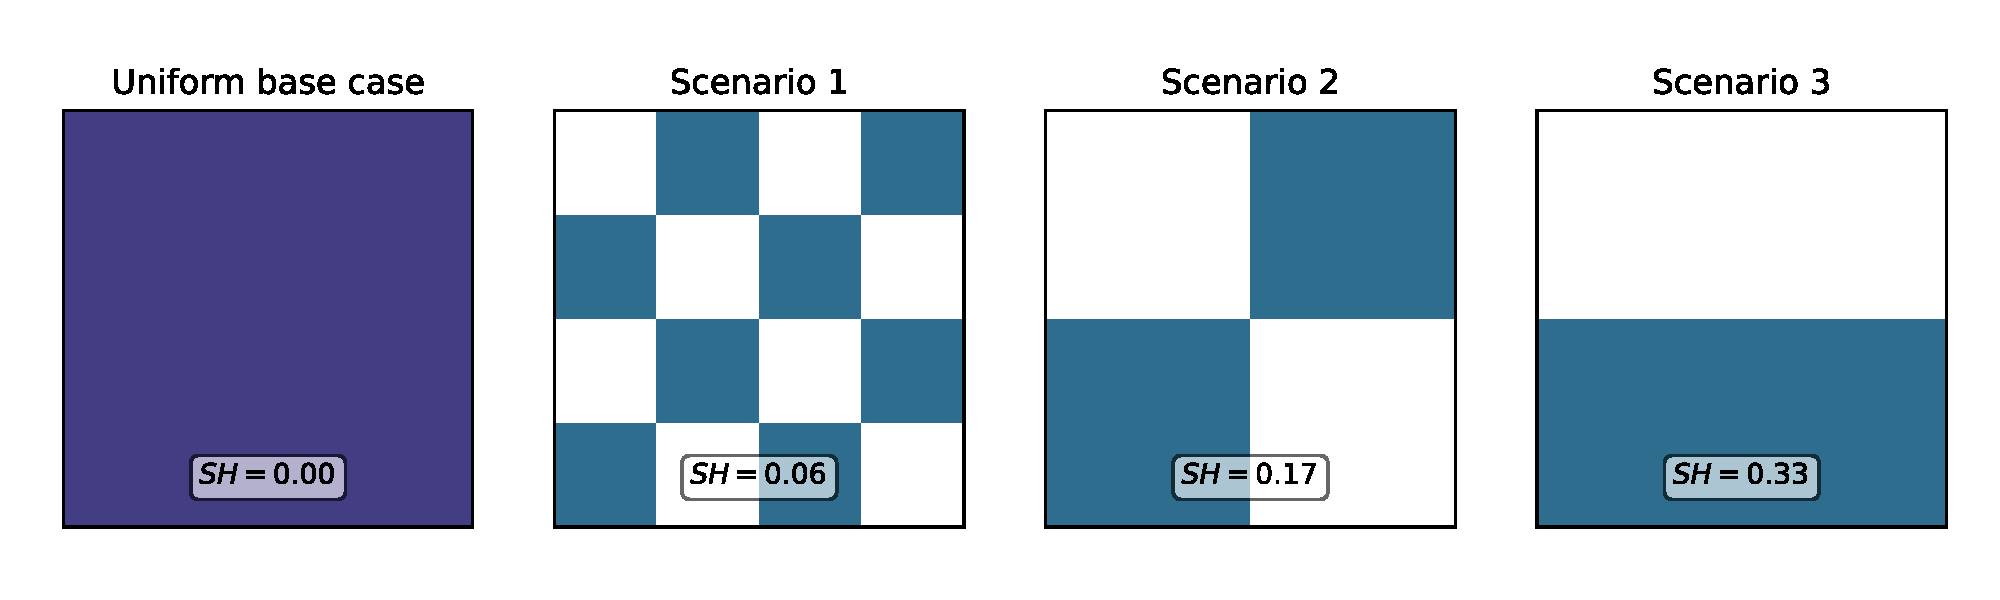
\includegraphics[width=\textwidth]{ozone-production-emiss-patterns.pdf}
	\caption{Emissions scenarios for ozone production simulations. The spatial heterogeneity of each emission scenario is listed in the lower portion of each scenario. For overlapping emissions cases, both NO$_x$ and VOCs are emitted in the same regions for each scenario indicted in blue. For non-overlapping emissions cases, NO$_x$ are emitted in blue regions while VOCs are emitted in white regions.}
	\label{fig:ozone-emission-patterns}
\end{figure}

We conduct seven simulations in total ranging in emissions spatial heterogeneity and the spatial colocation (or segregation) of precursor species responsible the production of ozone. Emissions scenarios are shown in Figure \ref{fig:ozone-emission-patterns}. The first simulation, named the uniform base case scenario, is characterized by uniform emissions of all compounds across the computational domain ground level. The uniform base case has a spatial heterogeneity equal to zero. This scenario represents the emissions across a single grid cell in a lower resolution model, such as a regional or global climate model, where emitted species are both uniform and dilute. Thus, results for simulations with higher emissions heterogeneity are compared against the uniform base case to quantify the structural uncertainty in ozone concentrations resulting from the assumption of uniform, dilute emissions characteristic of coarser resolved models that do not adequately resolve the true emissions spatial heterogeneity.  

Emission scenarios 1-3 are checkerboard patterns with increasing spatial heterogeneity. For each emissions scenario, we conduct two simulations: one run where precursors for ozone production, NO$_x$ and VOCs, are emitted in the same region (referred to as ``overlapping" emissions cases) and an additional run where the emission of NO$_x$ and VOCs are fully segregated (referred to as ``non-overlapping" emissions cases).

\section{Results}

\hl{NOTE: The simulations that I ran last summer were 1 hour in duration and emissions started at t=0, such that there was no initial spin up period prior to the release of emissions. I there there may also have been some issues with the emission rates (potentially) that led to very high O3 values, higher than typical of even polluted urban regions.}

\hl{Note that precursors are emitted into a background uniform concentration of 50 ppb as specified by the urban plume gas phase initial conditions,}

\hl{I think if I can show that the segregation intensity of VOCs and NOx is nearly 0 at t=60 min for even the most heterogeneous case then its a bit more justifiable to focus on only the first 1 hour.} Maybe? This is not so true for the nonoverlapping emissions though.

\subsection{Ozone cross sections}

\hl{ARM caption for cross sections: Snapshots of ozone mixing ratios in the x-y plane at approximately halfway up the boundary layer. Overlapping precursor emissions (top) result in larger ozone formation compared to non-overlapping precursor emissions (bottom).}

\begin{figure}[h]
    \centering
    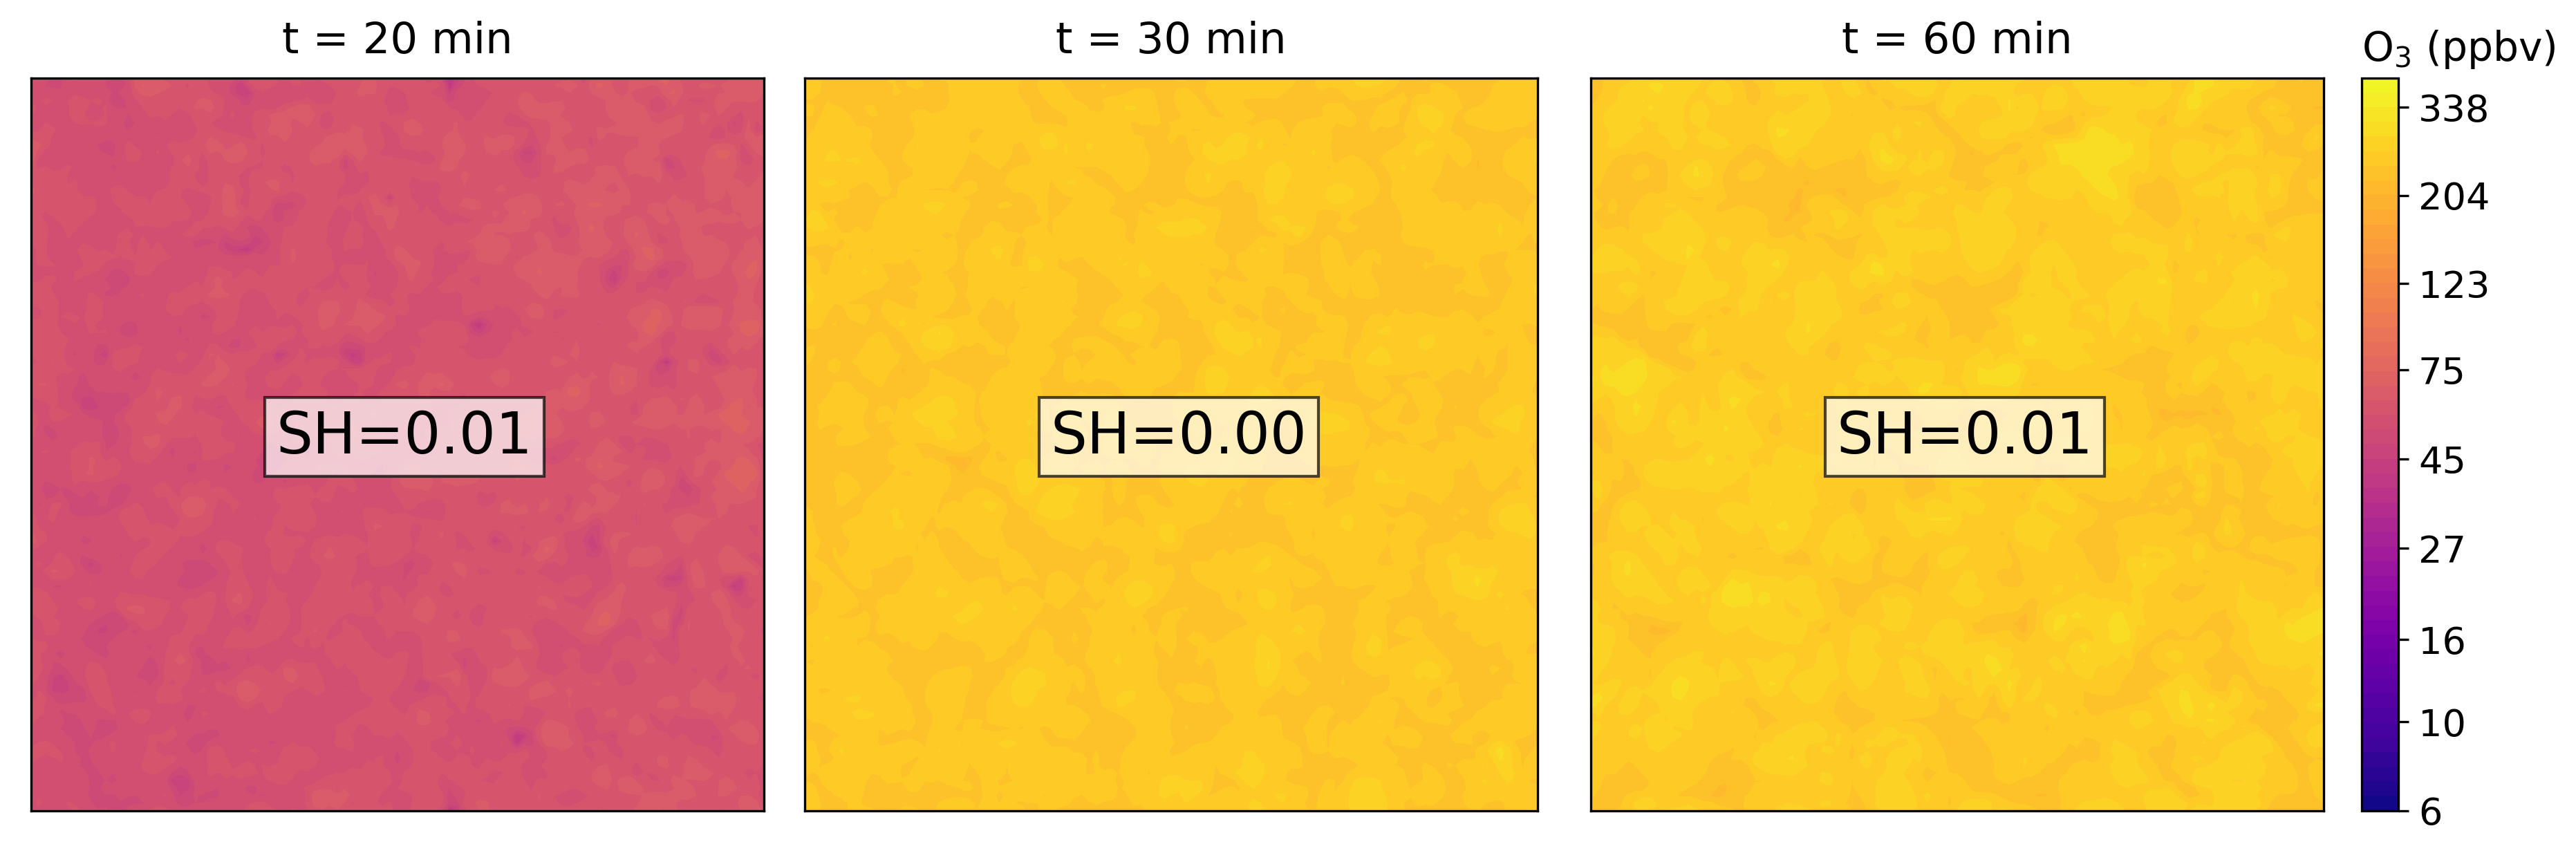
\includegraphics[width=\textwidth]{figures/ozone_cross_section_basecase_overlapTrue.png}
    \caption{Uniform base case}
    %\label{fig:aero_ic_dist}
  \end{figure}

\begin{figure}[h]
  \centering
  \begin{subfigure}
    \centering
    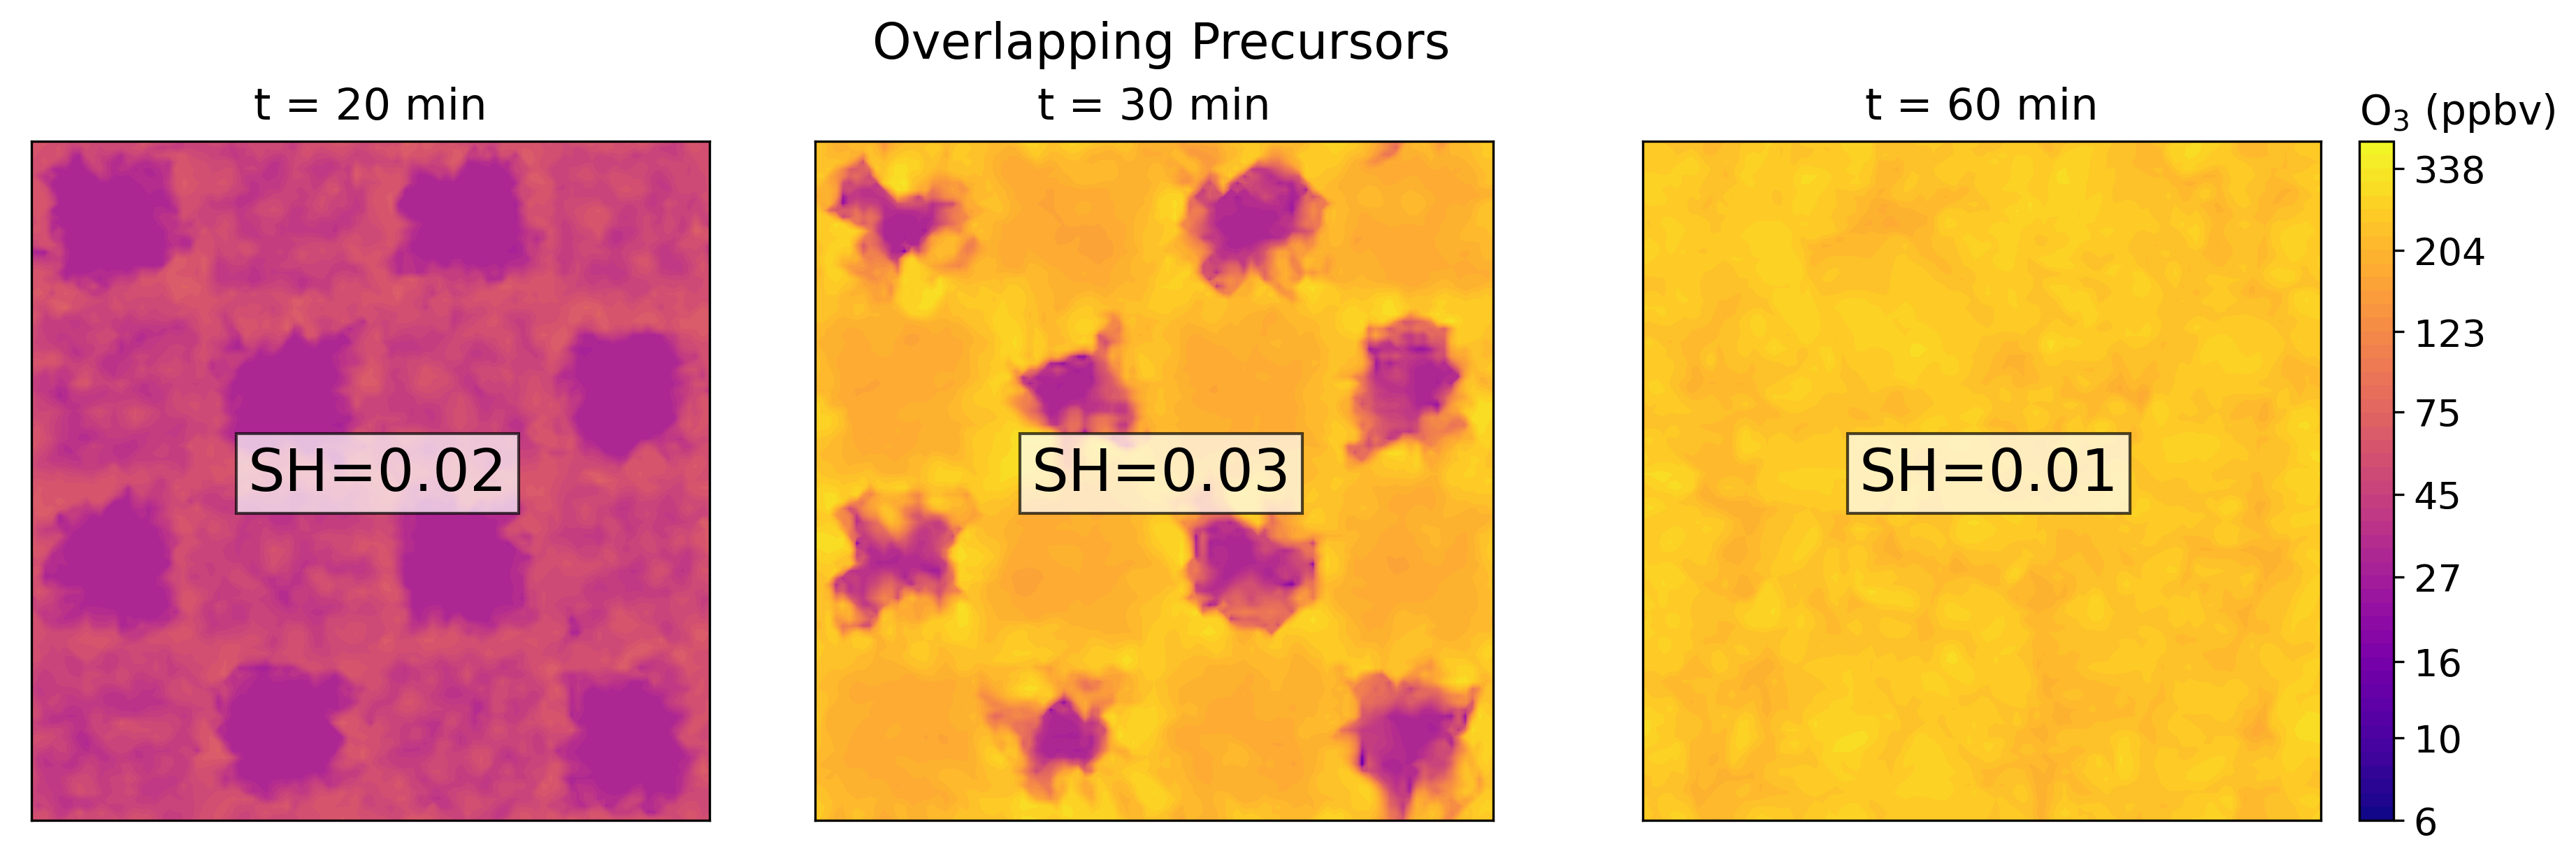
\includegraphics[width=\textwidth]{figures/ozone_cross_section_fx2fy2_overlapTrue.png}
    \caption{Scenario 1}
    %\label{fig:aero_emiss_dist}
  \end{subfigure}
     \vspace*{5mm} 
  \begin{subfigure}
    \centering
    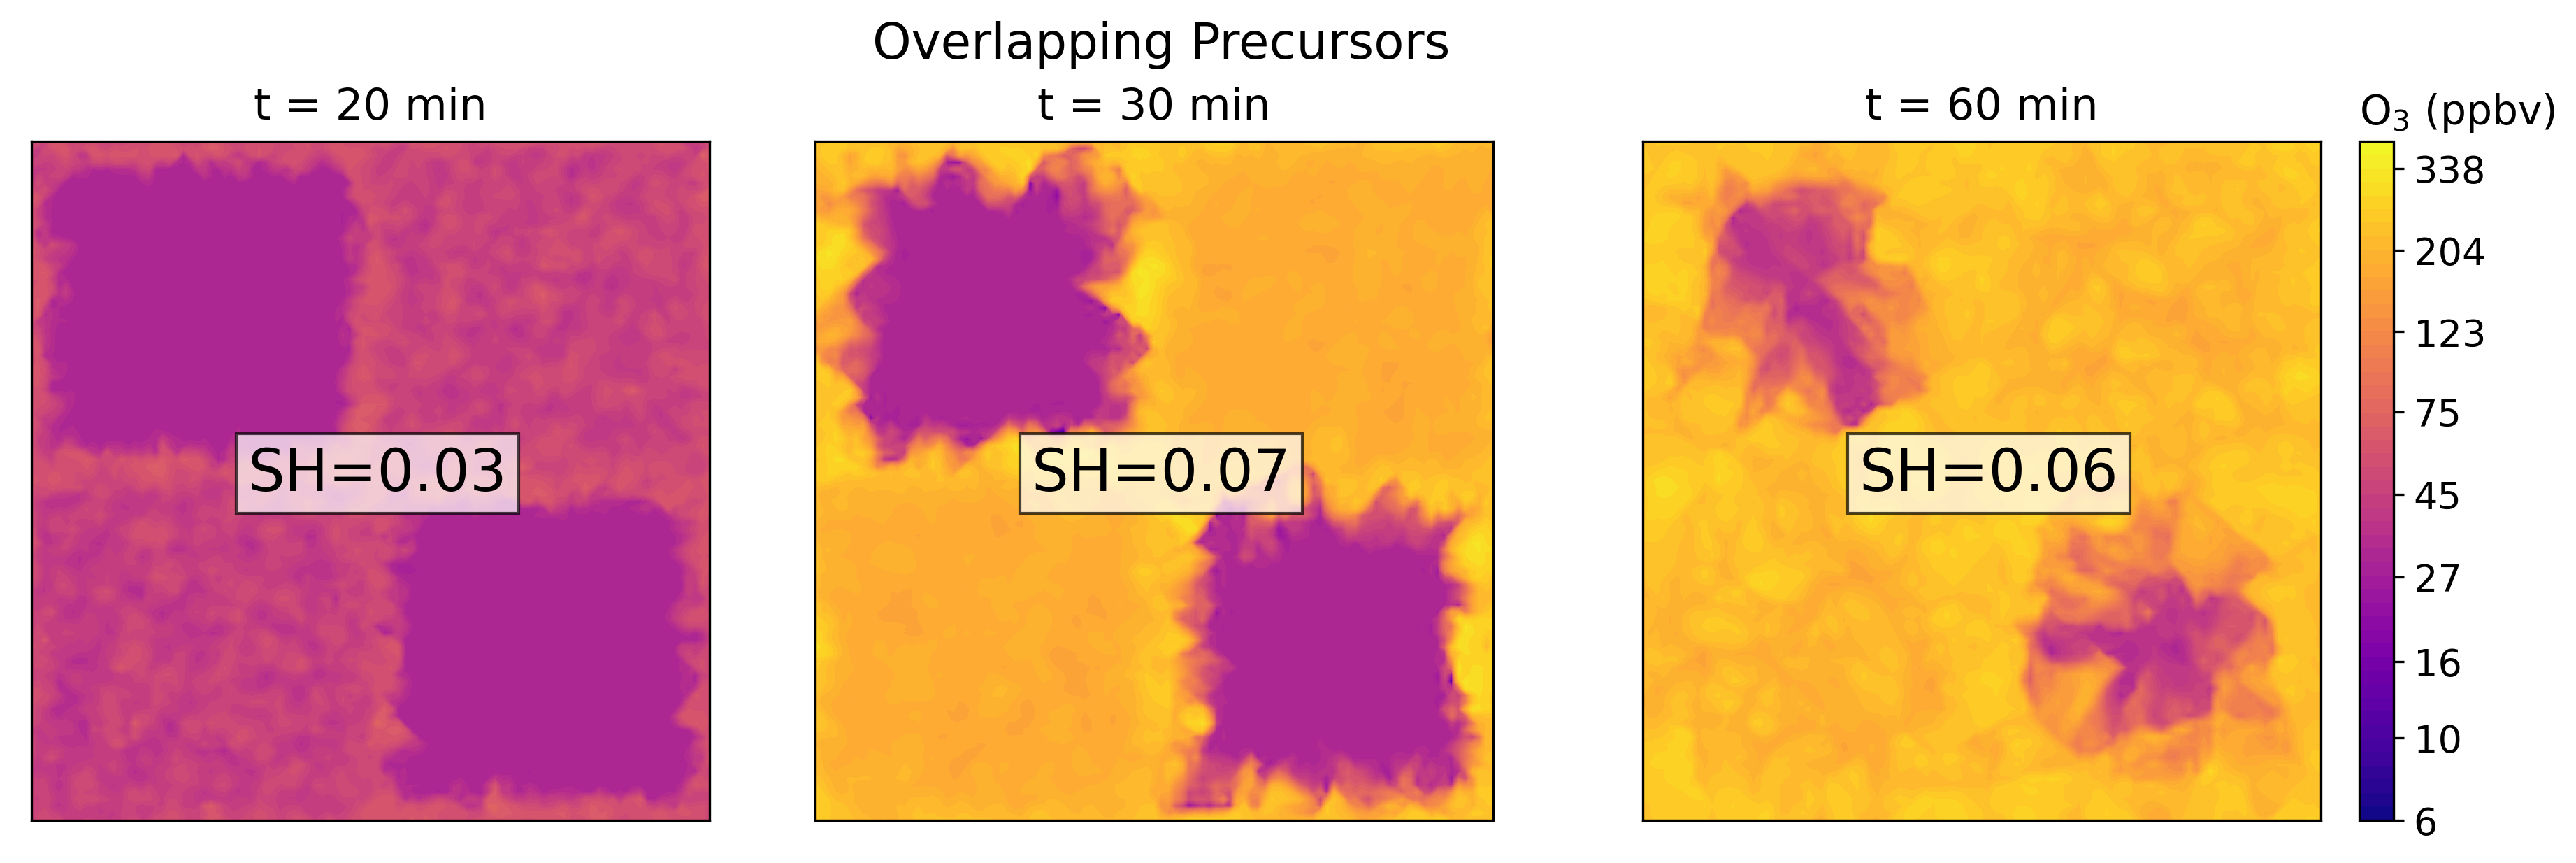
\includegraphics[width=\textwidth]{figures/ozone_cross_section_fx1fy1_overlapTrue.png}
    \caption{Scenario 2}
    %\label{fig:aero_emiss_dist}
  \end{subfigure}
   \vspace*{5mm} 
  \begin{subfigure}
    \centering
    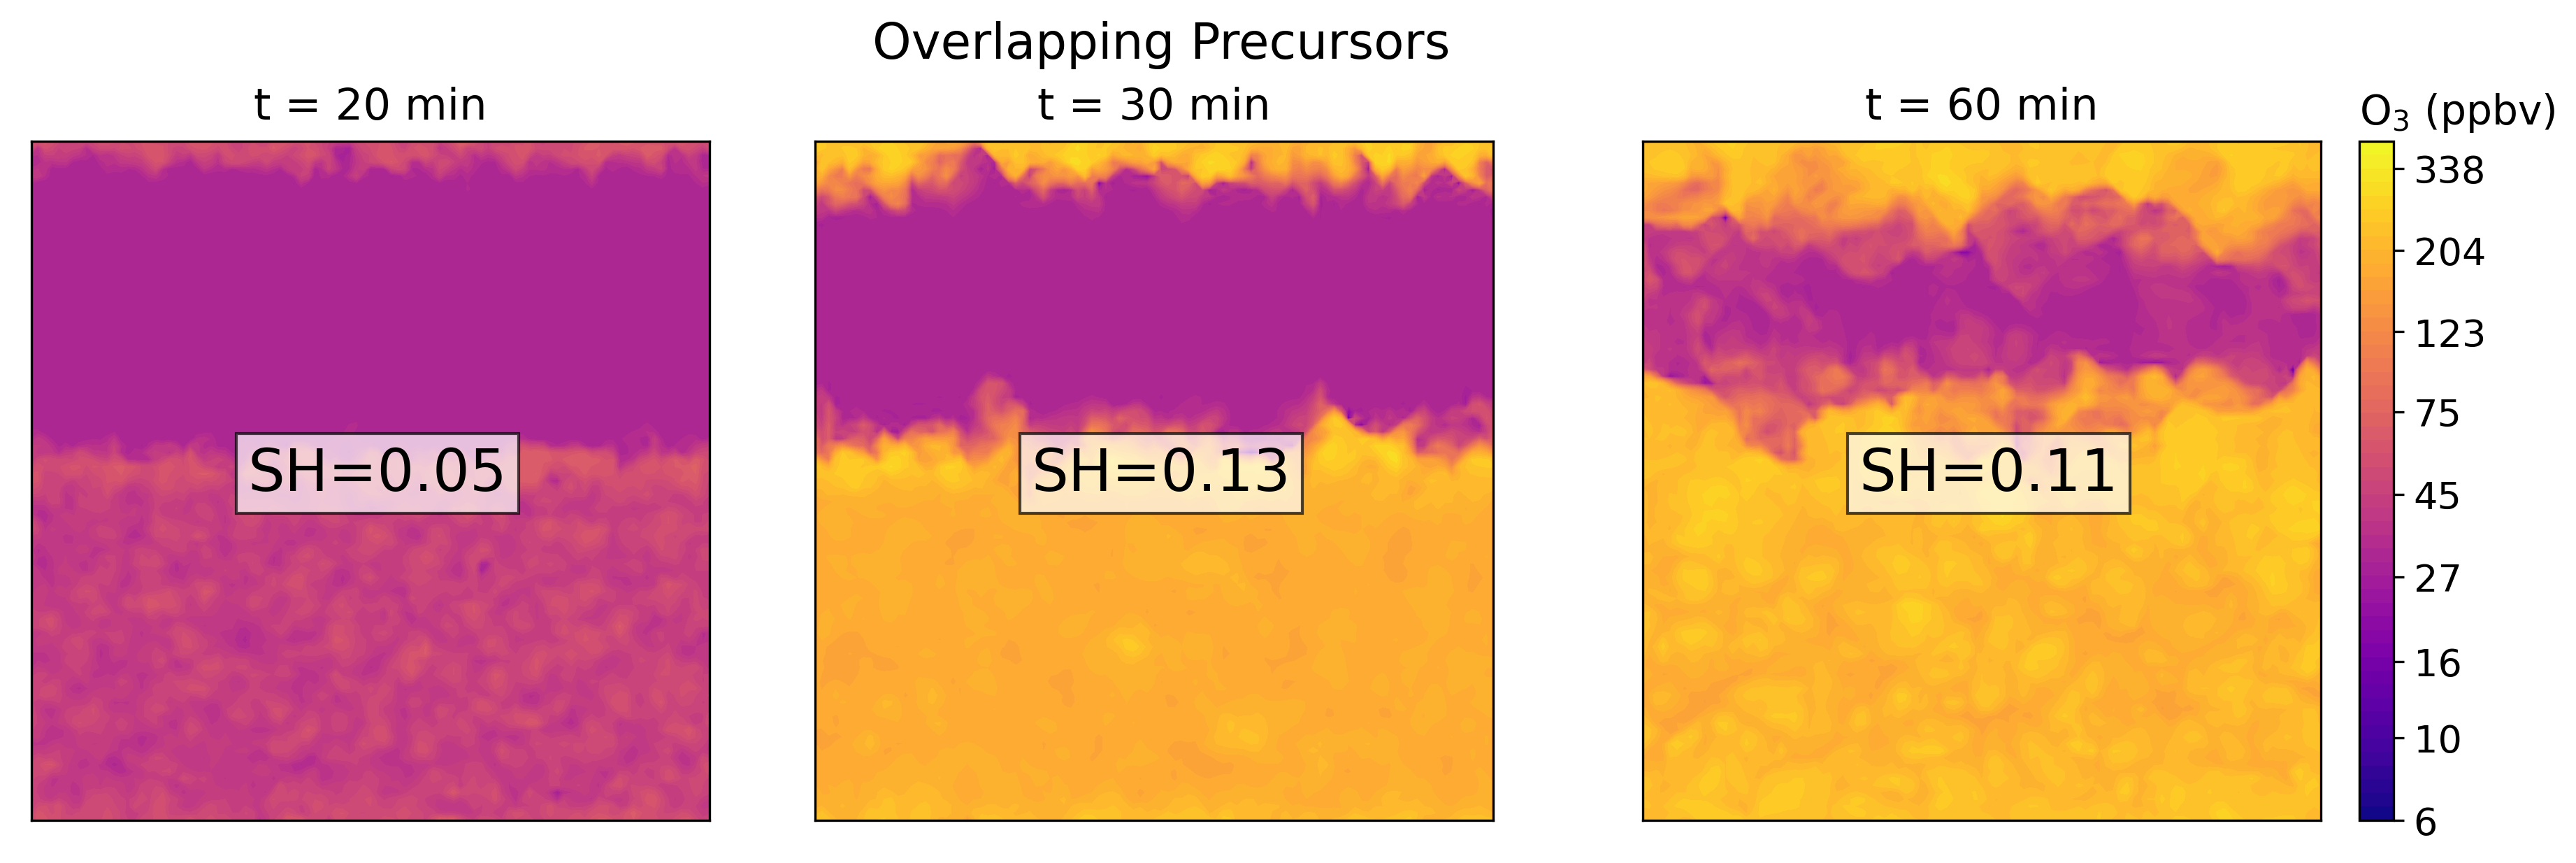
\includegraphics[width=\textwidth]{figures/ozone_cross_section_fx1fy0_overlapTrue.png}
    \caption{Scenario 3}
    %\label{fig:aero_emiss_dist}
  \end{subfigure}
\end{figure}

\begin{figure}[h]
  \centering
  \begin{subfigure}
    \centering
    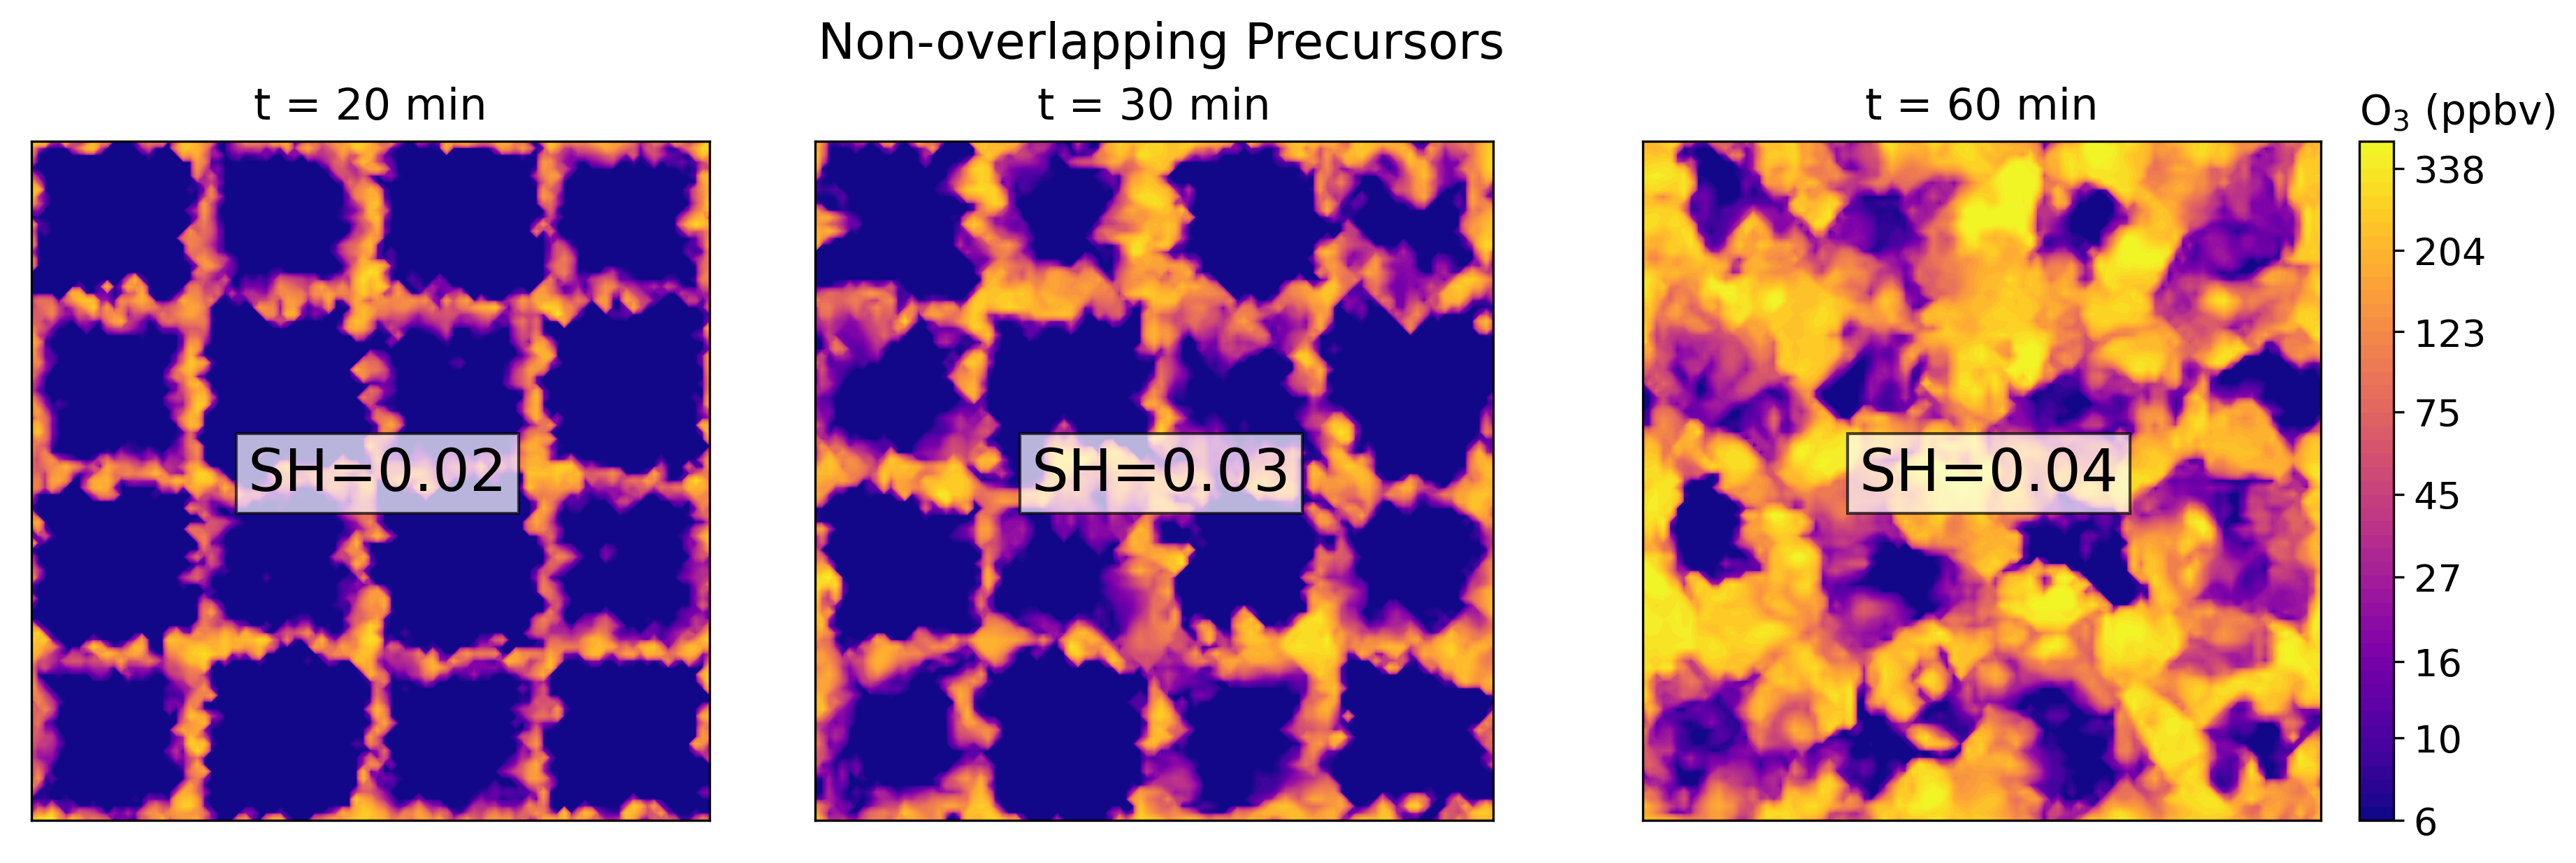
\includegraphics[width=\textwidth]{figures/ozone_cross_section_fx2fy2_overlapFalse.png}
    \caption{Scenario 1}
    %\label{fig:aero_emiss_dist}
  \end{subfigure}
     \vspace*{5mm} 
  \begin{subfigure}
    \centering
    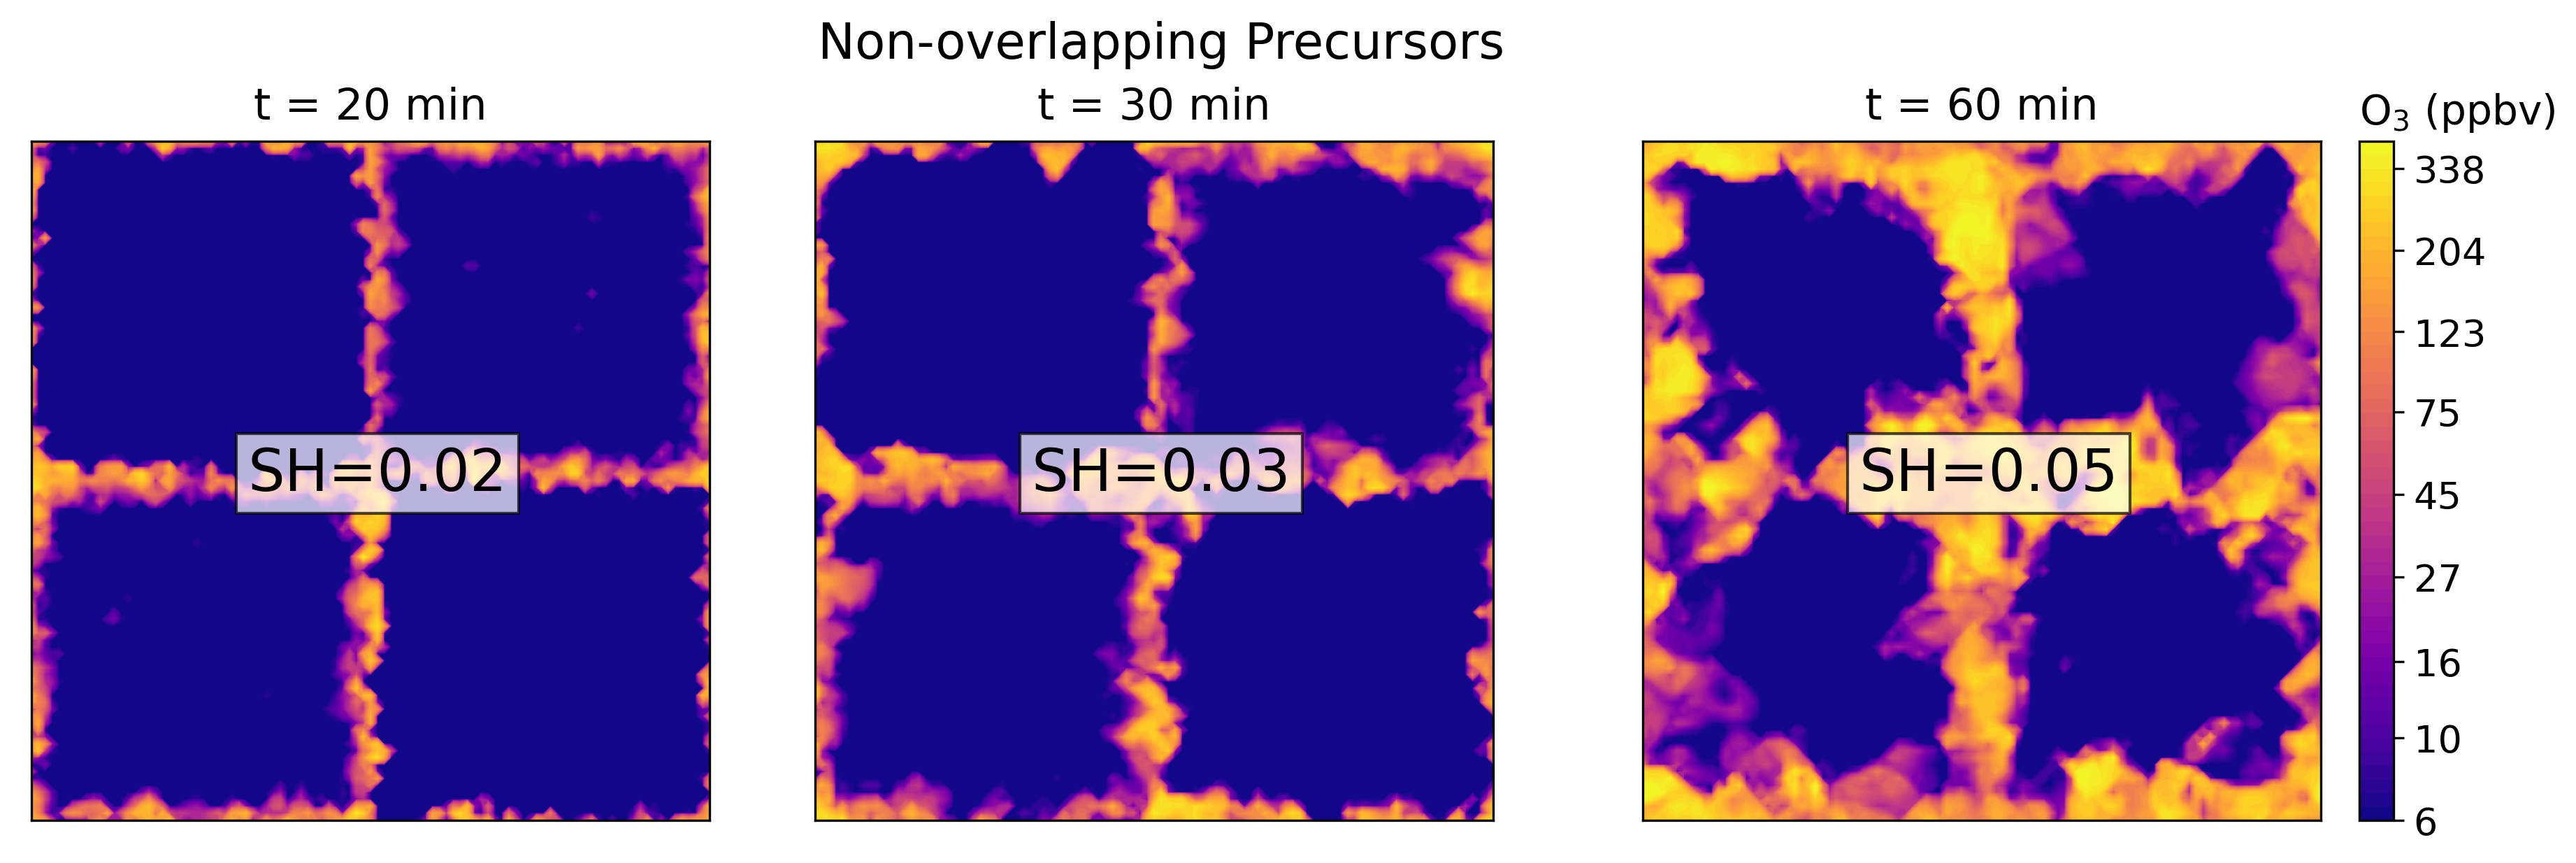
\includegraphics[width=\textwidth]{figures/ozone_cross_section_fx1fy1_overlapFalse.png}
    \caption{Scenario 2}
    %\label{fig:aero_emiss_dist}
  \end{subfigure}
   \vspace*{5mm} 
  \begin{subfigure}
    \centering
    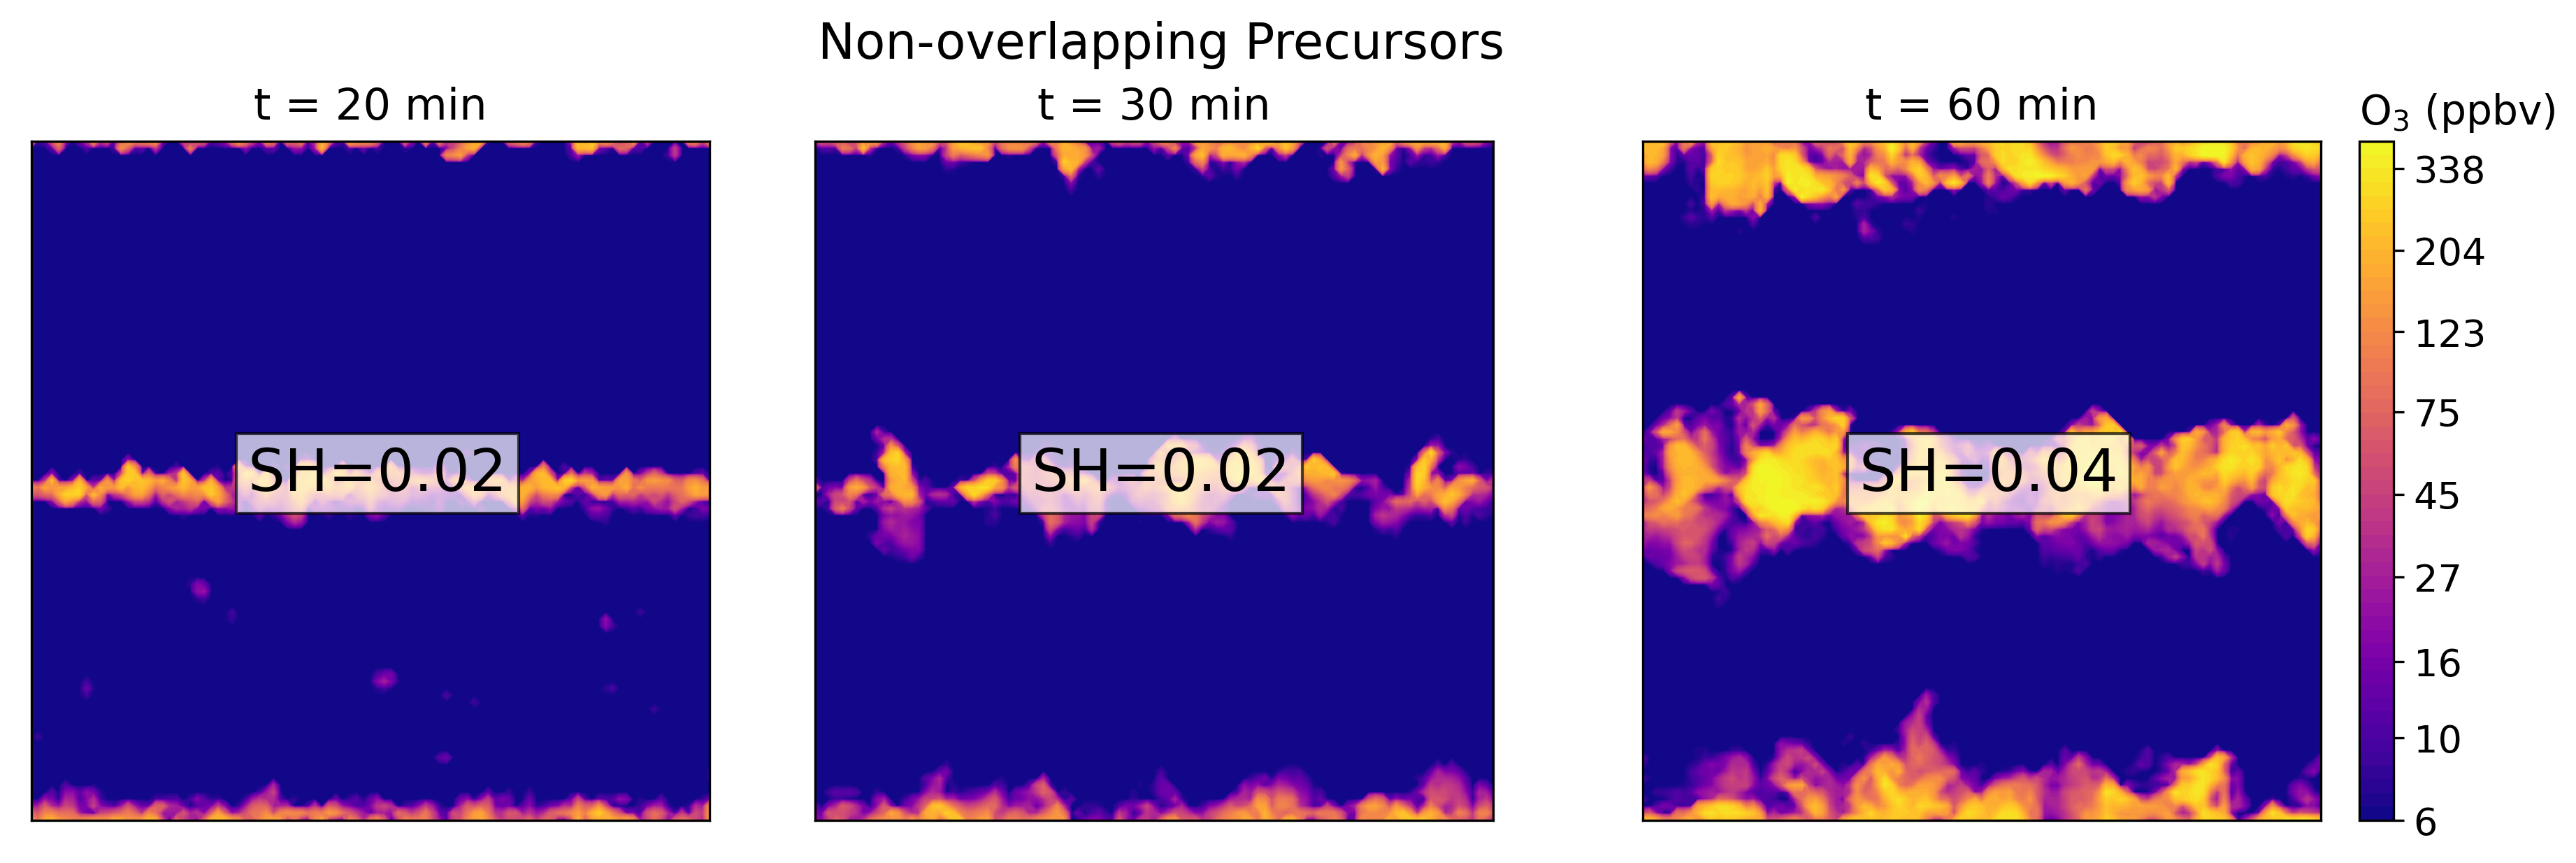
\includegraphics[width=\textwidth]{figures/ozone_cross_section_fx1fy0_overlapFalse.png}
    \caption{Scenario 3}
    %\label{fig:aero_emiss_dist}
  \end{subfigure}
\end{figure}

%\subsection{Segregation intensity}

\subsection{Spatial heterogeneity of ozone and its precursors}

\begin{figure}[h]
    \centering
    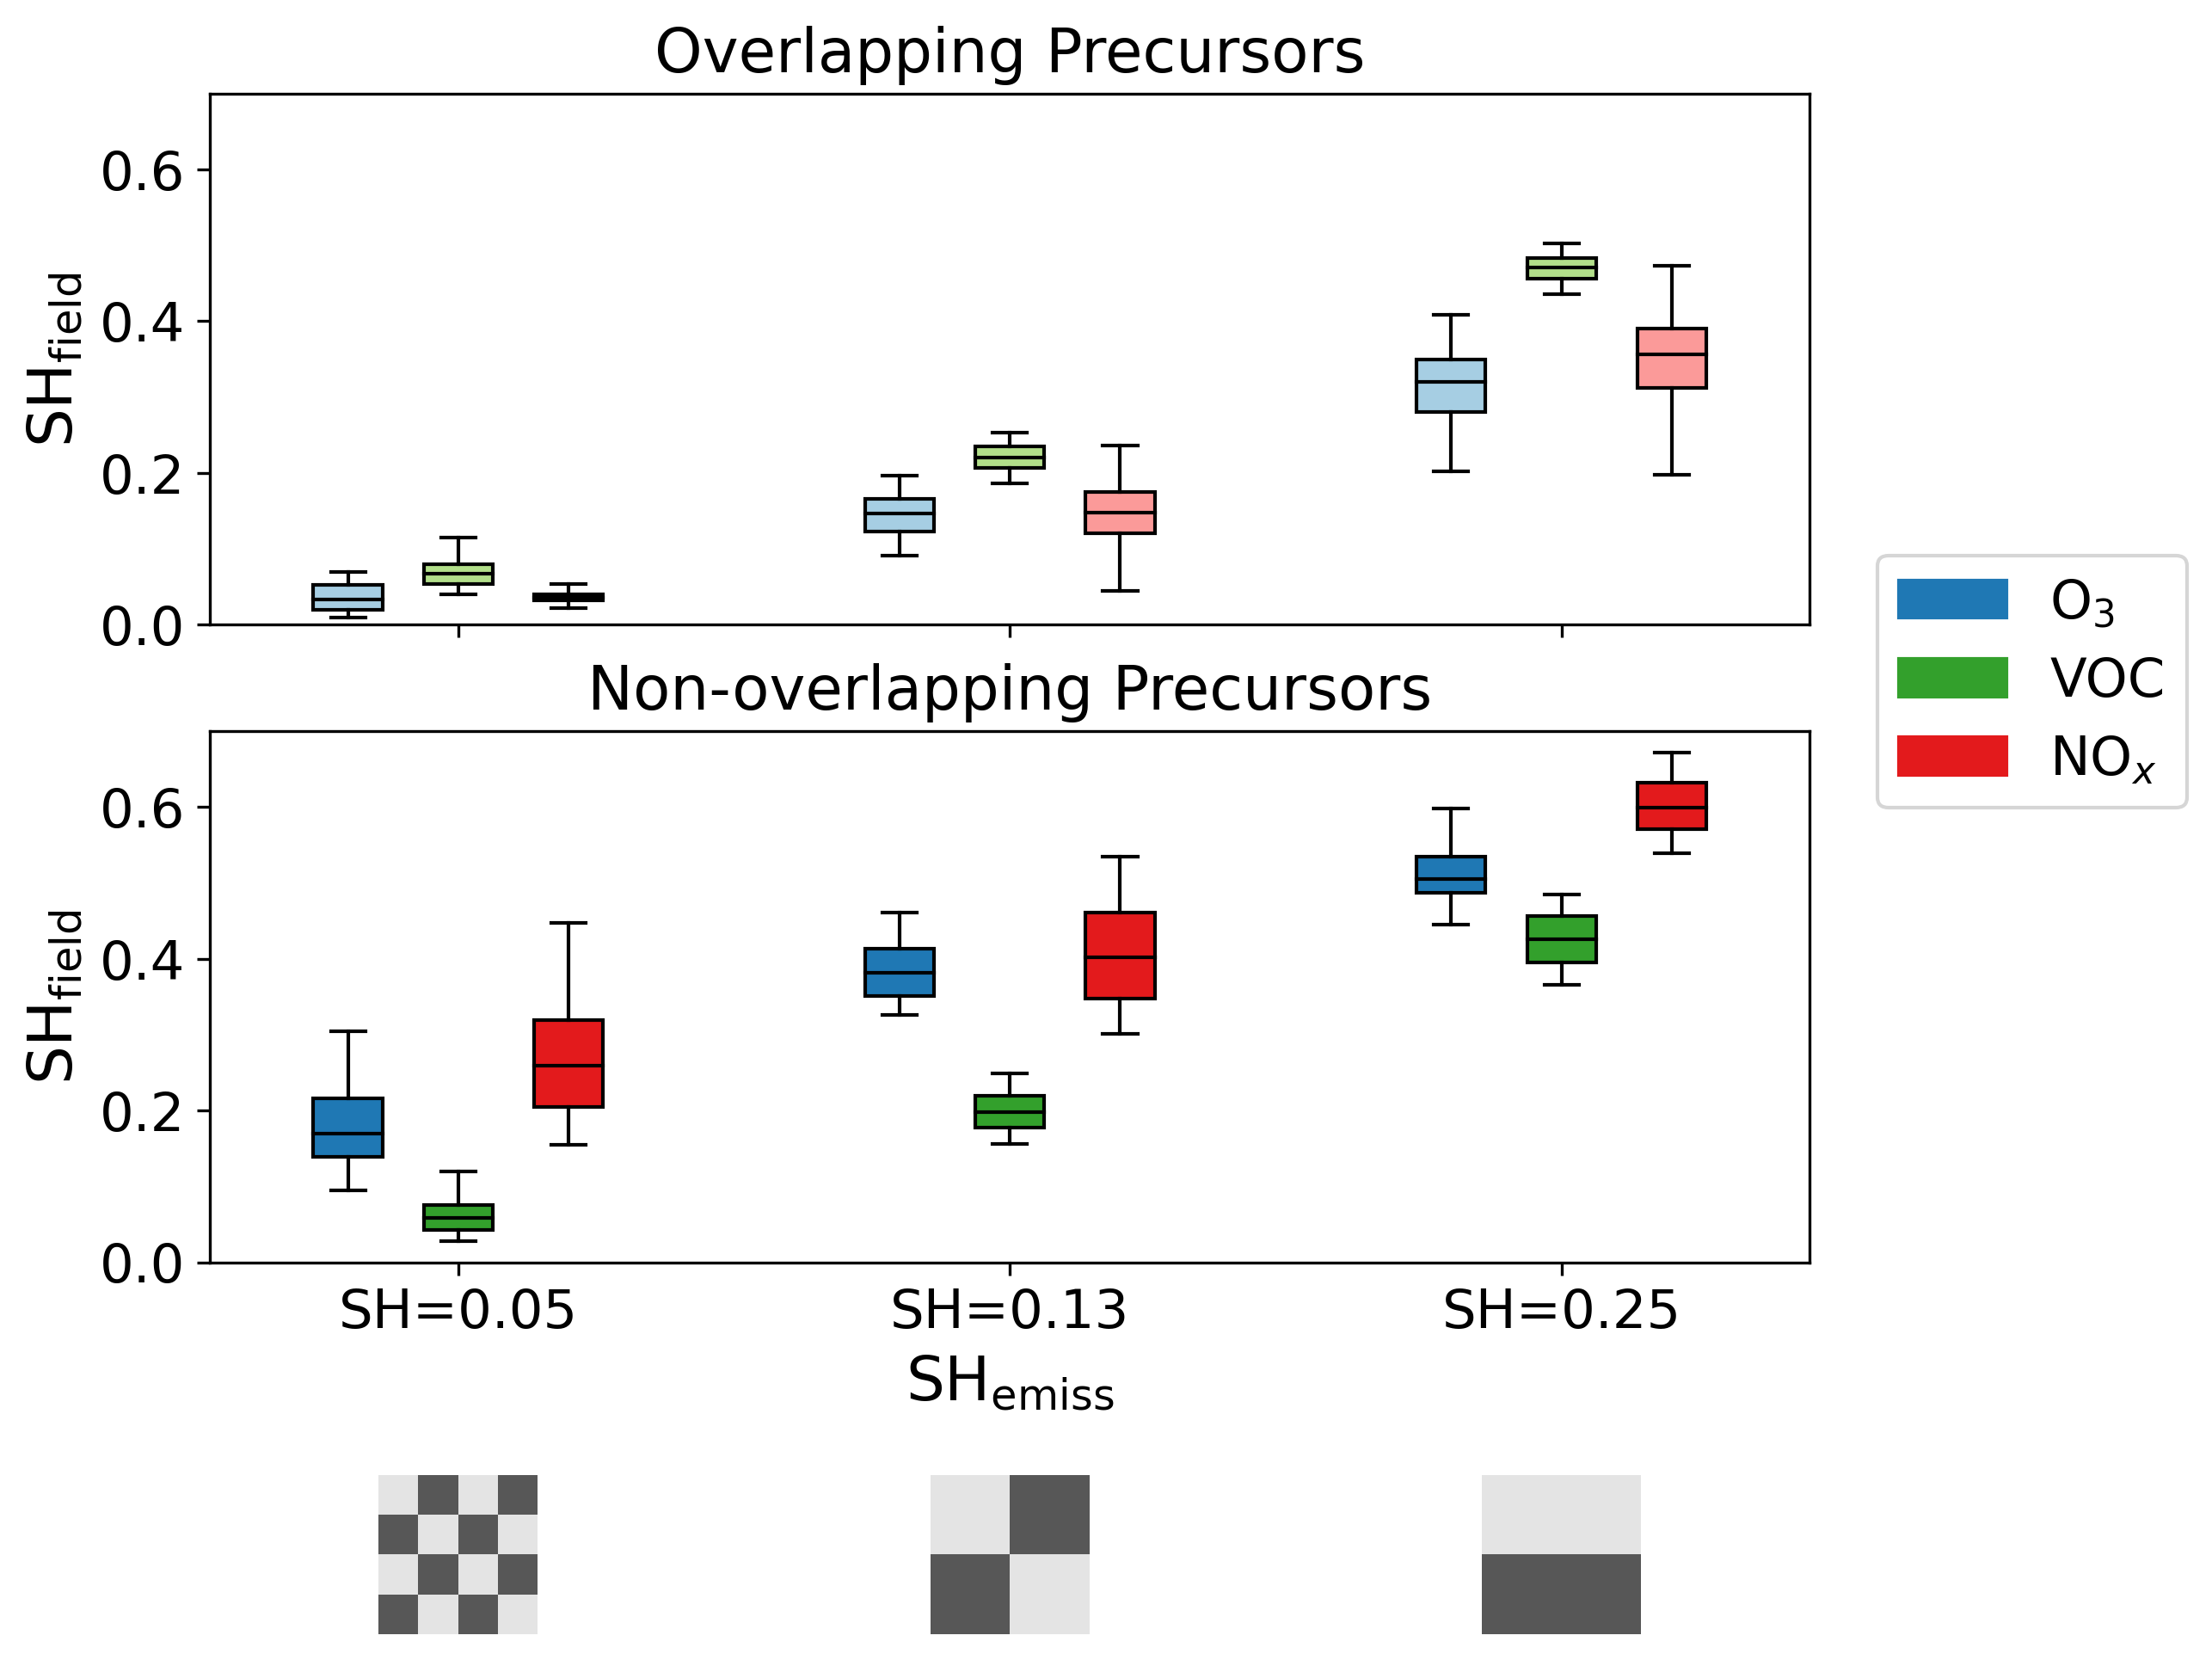
\includegraphics[width=\textwidth]{figures/field-SH-vs-emiss-SH-two-rows.png}
    \caption{\hl{Via ARM poster:} Relationship of SH of emissions and SH of concentration fields for the example of the directly emitted species NOx and VOC and the secondarily formed species ozone. SH of the concentration fields generally increases with increasing SH of the emissions. SH for NOx and ozone is larger for overlapping precursors compared to non-overlapping precursors.}
    %\label{fig:aero_ic_dist}
  \end{figure}

\subsection{Structural uncertainty in ozone production}

\begin{figure}[h]
    \centering
    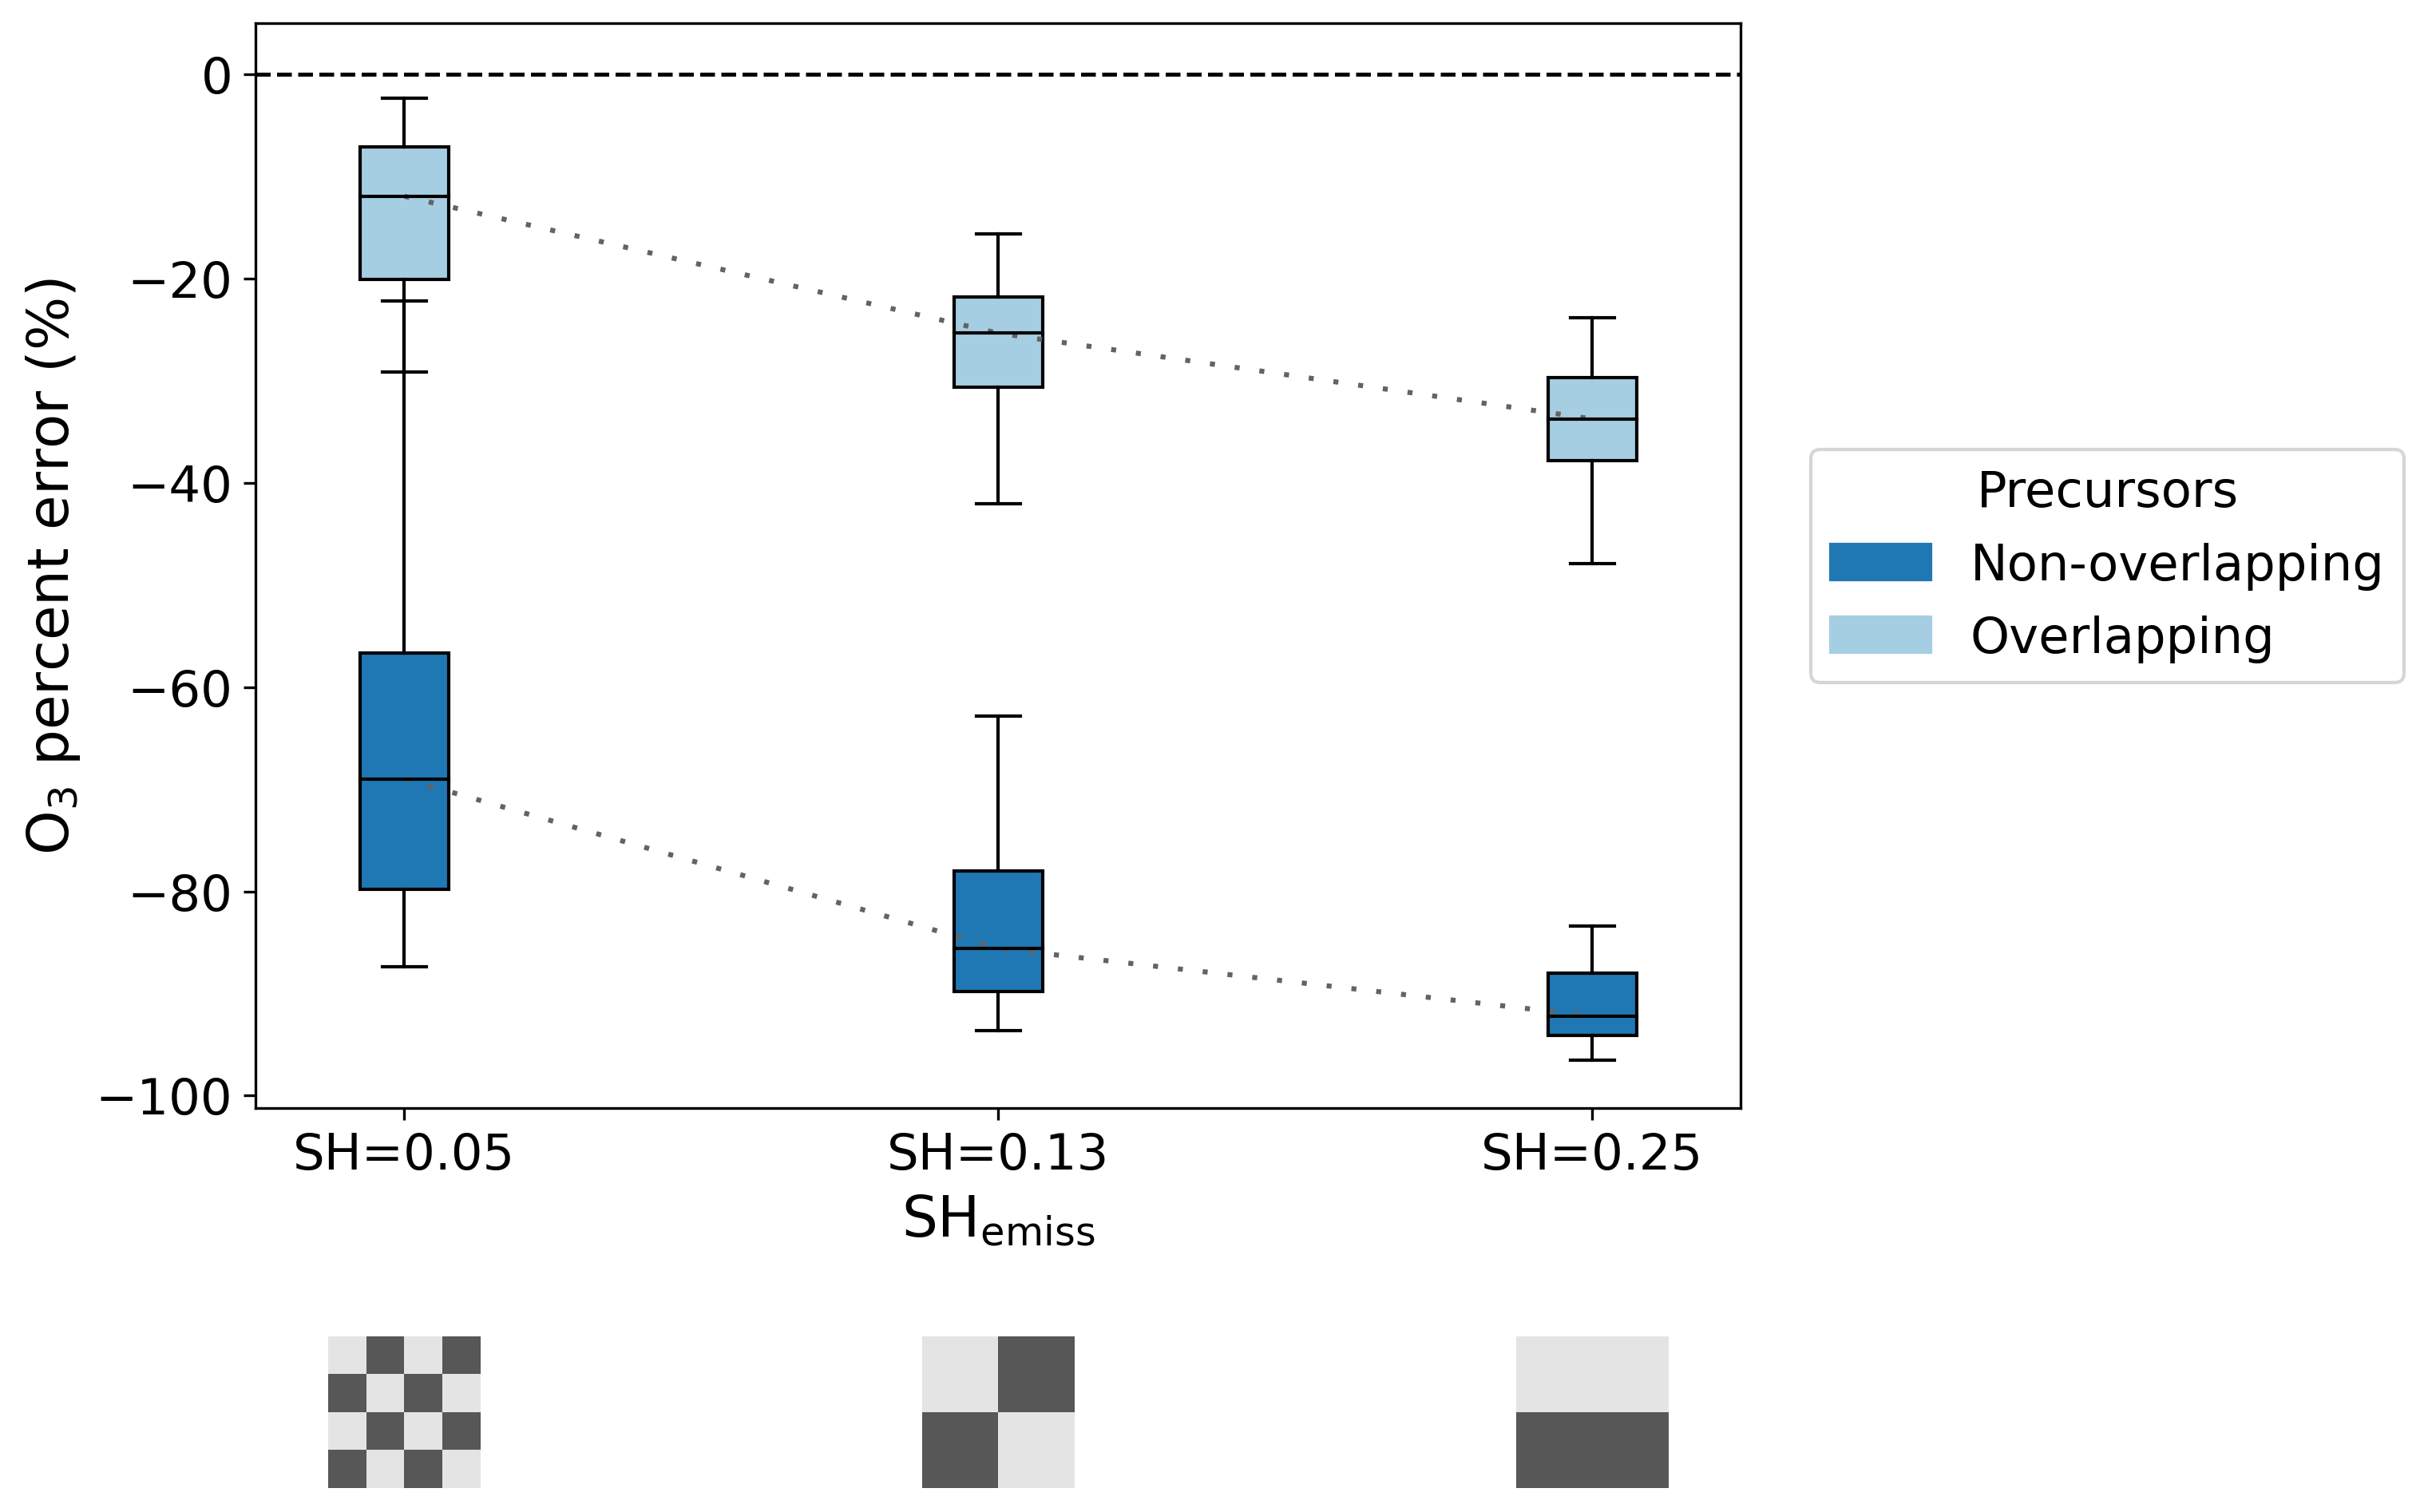
\includegraphics[width=\textwidth]{figures/O3-percent-err-vs-emiss-SH.png}
    \caption{\hl{Via ARM poster:} Deviation of ozone concentration from case with uniform NOx and VOC emissions. Larger SH in emissions and overlapping emissions lead to larger deviations.}
    %\label{fig:aero_ic_dist}
  \end{figure}
  
\section{Discussion}

\hl{This either goes here or in the introduction..}
\begin{itemize}
\item Worth noting at some point past studies that have evaluated the production of ozone in LES as well as some studies that investigate the impacts of spatial het. on ozone production (Initial studies investigated idealized interactions between turbulence and ozone chemistry in the PBL, more recent studies have branched into region-specific studies to investigate impacts of spatially heterogeneous emissions and turbulence-chemistry interactions on local ozone production).
\begin{itemize}
\item \cite{schumann_large-eddy_1989} Idealized LES of boundary layer - investigate binary reactions (such as those typical of ozone production) with varying reaction rates. For rates typical of ozone-nox reactions, the mechanism is significantly impacted by turbulence.
\item \cite{sykes_large-eddy_1992} Idealized LES of boundary layer - investigate turbulence chemistry interactions on ozone chemistry, particularly focused on the removal mechanism oxidizing NO to NO2 + O2. Find that the production rate of NO2 is highly dependent on the turbulent mixing of the plume. They show that the turbulence segregation coefficient can be approximated as uniform in a emitted plume. 
%\item \cite{krol_effects_2000} Maybe?
\item \cite{auger_chemical_2007} (seems very similar to what I am doing here) LES of PBL over 10x10 km domain. Indicate that segregation is strongest in the first two hours - after 3 hours segregation is largely reduced due to efficient mixing in the PBL. 
\item \cite{zhong_modelling_2015} Similar to Zhong et al 2017, find that ozone production rate is reduced due to incomplete mixing.
\item \cite{zhong_large_2017} LES study of O3-NOx-VOC chemistry in urban street canyons characterized by high spatial variability in concentration gradients. NOx and HOx radicals were consumed to produce NO2 and O3. Segregation effect due to incomplete mixing reduces the production of NO2. 
\item \cite{wang_impact_2021}
\item \cite{wang_segregation_2022} Similar to wang 2023
\item \cite{wang_coupled_2023} Use of LES (WRF-Chem LES \hl{what chem mechanism?}) for urban (Hong Kong) emissions compared against mesoscale simulations, show that NOx is underestimated and O3 overestimated in mesoscale simulations when compared to LES, attributed to the higher spatial resolution of emissions and explicitly resolving turbulent transport.
\end{itemize} 
\end{itemize}




